\section{Ziel}
In diesem Versuch wird die Funktionsweise eines Geiger-Müller-Zählrohrs betrachtet.
Es werden die Kennlinien der Betriebsspannung und die Totzeit der gegebenen Apparatur ermittelt.

\section[Theorie]{Theorie\footnote[1]{Unter Verwendung von \cite{man:v703}.}}
Geiger-Müller-Zählrohre gibt es in verschiedenen Versionen.
Die meisten haben aber einen Metallzylinder einen Zählrohrdraht meist aus Wolfram. 
Der Zylinder ist mit einer dünnen Mylarfolie oder einem Glimmer verschlossen, welche gleichzeitig als
Eintrittsfenster dienen.
In der Kammer eingeschlossen ist ein Edelgas, welches mit Kohlenwasserstoffen versetzt ist.
Zwischen dem Draht un dem Zylinder ist eine Spannung angelegt.

Tritt ionisierende Strahlung in die Kammer ein, wird das Gasgemisch im Innern der Kammer ionisiert.
Durch die Angelegte Spannung werden die Ionen von zum Draht oder zum Zylinder hin beschleunigt.
Auf dem Weg dahin können die Elektronen bzw. Ionen bei einer ausreichenden Spannung weitere Gasmoleküle ionisieren, sodass eine Kettenreaktion ausgelöst wird.
Das führt wiederum zu einer großen Anzahl an Ladungsträgern, die über einen Widerstand abfließen.
Da der Widerstand im Megaohmbereich liegt führt dieser Prozess zu einem Abfall in der Spannung, der die Kettenreaktion dann unterbricht.
Mit einem Verstärker kann dieser kurzzeitige Spannungsabfall in einem Zählgerät oder einem Oszilloskop gemessen werden.
Die Zeit dieses Spannungsabfalls wird auch Totzeit genannt, da keine weiteren Strahlungen während dieser Zeit gemessen werden können.

%% Vielleicht in die Durchführung diesen Teil:
In Abbildung \ref{fig:01_teo} ist der Aufbau der hier verwendeten Apparatur zu sehen.
\begin{figure}
    \centering
    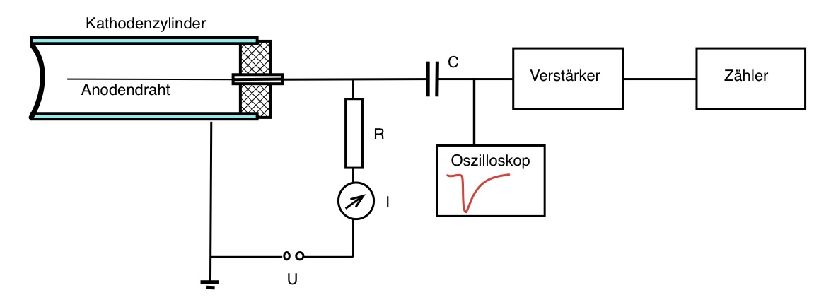
\includegraphics[width = 0.75\textwidth]{14_v703/Abbildungen/Seite 2.pdf}
    \caption{Aufbau der Messapparatur \cite{man:v703}}
    \label{fig:01_teo}
\end{figure}
%% bis 
\begin{figure}
    \centering
    \input{14_v703/Inhalte/A_Test.pdf_tex}
    \caption{Die Zählrohrcharakteristik.}
\end{figure}

Die Zählrate des Geiger-Müller-Zählrohrs hängt von der Betriebsspannung ab.
Diese Abhängigkeit wird Zählrohrcharakteristik genannt. 
Folgende Bereiche sind dabei relevant
\begin{itemize}
    \item \textbf{Rekombination:} Bei einer niedrigen Betriebsspannung werden keine Zerfälle gemessen.
    Die gebildeten Ionen können sich auf dem Weg zum Anodendraht wieder mit Elektronen zu neutralen Atomen verbinden.
    \item \textbf{Ionisationskammer:} Ab einer gewissen Spannung erreichen alle Elektronen bzw Ionen die Elektroden, und es wird ein Sättigungsstrom erreicht.
    In diesem Bereich kommen nur die Elektroden und Ionen an, die direkt von der Strahlung erzeugt werden.
    \item \textbf{Proportionalitätsbereich:} Wenn die Spannung weiter erhöht wird, können die Elektronen mit Stoßionisation weitere Elektronen Ionen Paare erzeugen. 
    Dieser Prozess passiert in der Nähe des Anodendrahts sehr häufig was zu einer Verstärkung des Spannungsabfalls um einen Faktor der Größenordnung \num{10^3} führt.
    % Die Verstärkung ist hierbei abhängig von der Art der Strahlung
    \item \textbf{} 
    \item \textbf{} 
\end{itemize}


\section{Vorbereitung}
In diesem Versuch wird eine \ce{^{204}Tl}-Quelle verwendet.
